\chapter{Results\label{results}}
% information about chapter
This chapter employes the data extracted from the set of primary literature, available in this thesis' repository\footnotemark[1] under the name of \texttt{stage1-licenses.md}, utilizing the methods outlined in \hyperref[methods]{Chapter 2} to address the research questions. Firstly, a summary of the general statistics collected and aggregated from the studies is presented. Following that, an analysis of the data is performed to provide answers to each of the research questions.

% note about publication year and number of literature
To begin with, the publication year was not limited and could not have been limited in a rigorous way. Almost all of the public software licenses came from different sources although they were listed in the five license listing sites. To give a rough estimate, one of the earliest public software license aiming for legal compliance was the original GPL from 1989 \citep{license-history}. The search was carried out by web scraping all of the licenses from the five license listing sites without any filters to the attributes of the licenses. The initial search results included 1057 public licenses, but after the exclusion and quality criteria of software-only license scope, the final resulting dataset was reached.

% statistical overview
Given the large starting dataset, a simple statistical overview of the literature was generated and is presented in \hyperref[fig:3-1]{Figure 3.1} and \hyperref[fig:3-2]{Figure 3.2} with the full list of literature available in this thesis' repository\footnotemark[1] under the name of \texttt{stage1-licenses.md}.
\begin{figure}
	\centering
	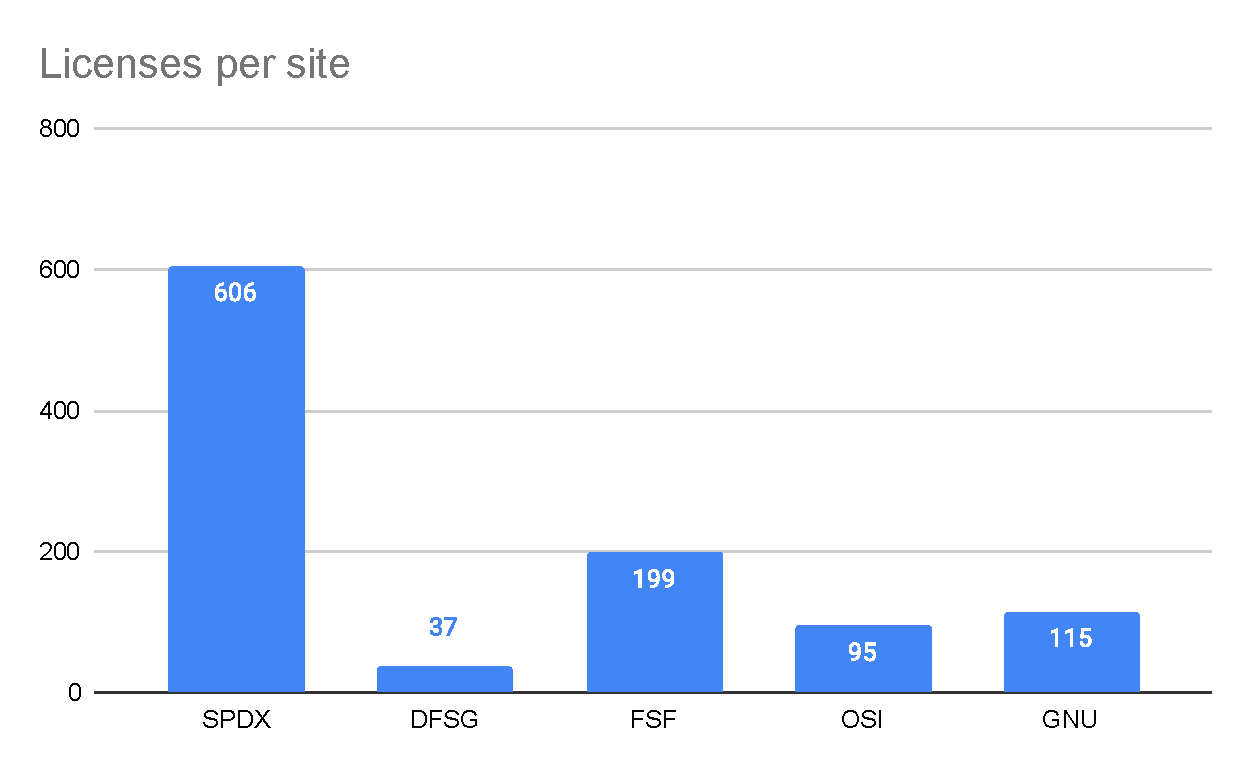
\includegraphics[scale=0.76]{figures/figure-3-1.pdf}
	\caption{Licenses per site totaling in 1057 licenses}
	\label{fig:3-1}
\end{figure}
\begin{figure}
	\centering
	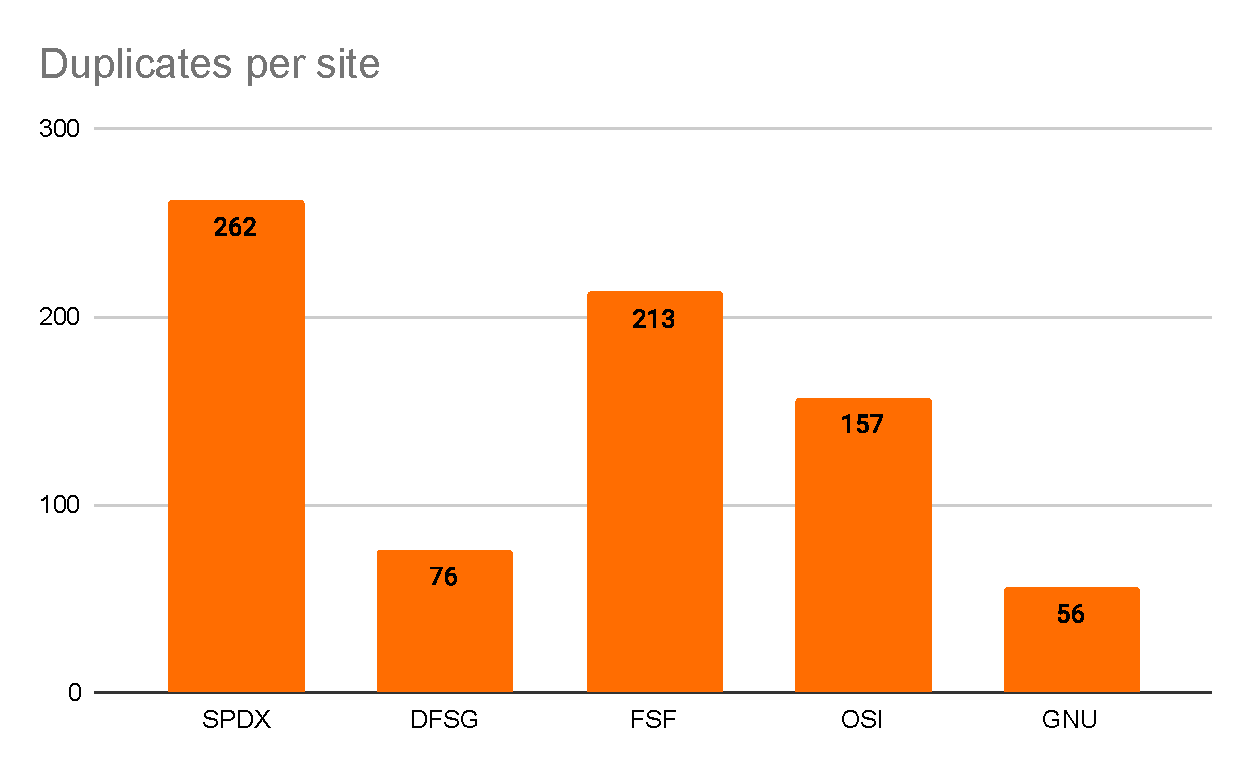
\includegraphics[scale=0.76]{figures/figure-3-2.pdf}
	\caption{Duplicates licenses per site totaling in 1057 licenses}
	\label{fig:3-2}
\end{figure}
The statistics highlight some immediate observations, such as the volume differences between the five sites and how the initial volume does not correlate to the number of duplicate one site holds compared to the four others.
\footnotetext[1]{\url{https://github.com/akirataguchi115/mscthesis/}}

% recap search process (todo remove redundant repetition)
After establishing the quasi-gold standard and completing the preliminary study review outlined in \hyperref[methods]{Chapter 2}, we systematically searched for relevant literature using the five license listing sites. The resulting search findings were filtered through a set of inclusion/exclusion criteria, followed by an extensive evaluation of quality before the final step of manual review. The final collection of literature consisted of almost 600 licenses, for which we obtained and reviewed the complete texts while completing the data extraction form as presented in \hyperref[table:extraction]{Table 2.1}.

We observed the number of literature acquired is adequate to gain an representative overview of the field, which we will explore further in this chapter.

After this overview let us take a look into the specific research questions and their answers.

\section{Five license listing sites and their licenses (RQ1)}
% spdx gave least headache
Only license listing site during the first phase of the search process that did not give too much trouble was the SPDX. This was mostly be due to the table format used in that particular license listing site, shortcode identifier being provided inside that table and that it seems that SPDX preserves many of the licenses regardless of legal validity, superseding licenses or voluntary retirement.

% the rest listing sites gave headache
The four other listing sites were more problematic to scrape. An example of DFSG is that for example for the license ''Licence Art Libre (Free Art License)'' I had to just use the more commonly used shortcode \texttt{FAL} because the shortcode itself was not listed in DFSG. FSF used a Wiki as the base for the license listing site so there was plenty of missing and outdated data. For example the original \texttt{Python} license has the full text of just ''test'' which indicates a pure mistake or a placeholder from the FSF. OSI had licenses that were retired between the search stages one and two. For example \texttt{cvw} was listed during the initial web scraping of the five listing sites but during the full license text fetching from the public license database of ScanCode the original creator of \texttt{cvw}, MITRE had voluntarily retired their license from the OSI license listing site and was no longer found from the OSI license listing site even though the missing license was noted to be from the OSI in the spreadsheet. The license was found however under the shortcode \texttt{cvwl} from the ScanCode public license database. This specific issue could have been solved by using an internet archiver, which we will discuss further in \hyperref[discussion]{Chapter 4}. GNU for example listed licenses like \texttt{attpubliclicense} which pointed the full license text to reside in and FSF site but the full license text was empty. In this case we had to just use the comments made by GNU as the full license text in this thesis.

% tell more in validity threats
These are just individual examples of the level of maintenance appearing in the four other license listing sites and some other examples will be brought up later in the next chapter. This is because solving these problems also becomes more of a validity threat of the author regardless of the fact that this kind observation is a relevant result on its own in this thesis. When we count the number of license per listing site after search stage one we get 607 licenses from the SPDX, 38 from the DFSG, 200 from the FSF, 96 from the OSI and 116 from GNU. The distribution of licenses from the five listing sites is illustrated in \hyperref[fig:3-3]{Figure 3.3}.
\begin{figure}
	\centering
	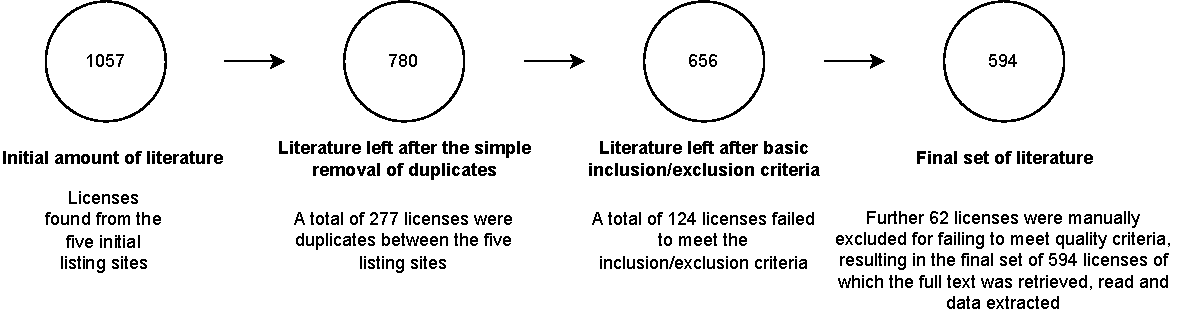
\includegraphics[scale=0.76]{figures/figure-3-3.pdf}
	\caption{Distribution of license across the listing sites}
	\label{fig:3-3}
\end{figure}
\section{Duplicates in license listing sites (RQ2)}
% note the number of duplicates per site
A total of 277 duplicates compared by exact shortcode after search stage one and 62 more duplicates were found after applying the exclusion criteria after search stage three. The intial 277 duplicates indicates some level of disagreement about the shortcodes between the five license listing sites. This is because these shortcodes are not treated unique across the listing sites. The following citation from GNU \citep{gnu:licenselist} about the \texttt{MIT} license demonstrates clearly the phenomenon affecting all five listing sites:
\begin{quote}
  ''Some people call this license 'the MIT License,' but that term is misleading, since MIT has used many licenses for software. It is also ambiguous, since the same people also call the X11 license 'the MIT License,' failing to distinguish them. We recommend not using the term 'MIT License.'
  
  The difference between the X11 license and the Expat license is that the X11 license contains an extra paragraph about using the X Consortium's name. It is not a big deal, but it is a real difference.''
\end{quote}
GNU calls the \texttt{MIT} license as the \texttt{Expat} license. A notable observation being here that the \texttt{MIT} license was used in approximately 45\% of repositories in 2015 \citep{github:licenseusage} and with 4.8 million unique Git pushers in 2024 with the \texttt{MIT} license used as the license for the source code making the \texttt{MIT} license the most used license in GitHub in all four quarters of 2024 \citep{github:innovation}. The same license was also used the most between the years 2020 and 2024 as can be seen in \hyperref[fig:3-4]{Figure 3.4}.
\begin{figure}
	\centering
	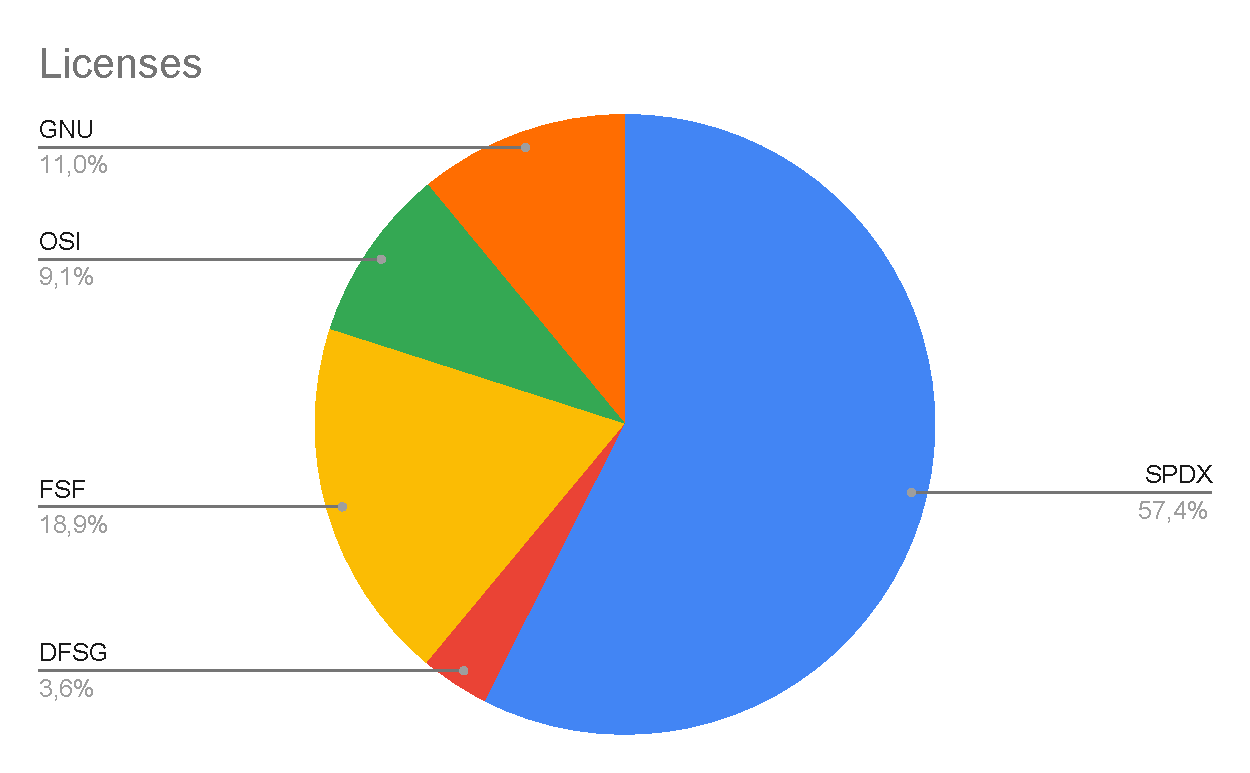
\includegraphics[scale=0.73]{figures/figure-3-4.pdf}
	\caption{License usage between years 2020 and 2024 in GitHub with MIT being the most used public software license every year}
	\label{fig:3-4}
\end{figure}
GNU demonstrates the same phemonemon of shortcode disagreement with the \texttt{GPL-3.0} license being either \texttt{GPL-3.0-only} or \texttt{GPL-3.0-or-later}, disagreeing with any other shortcode staten by the other four listing sites \citep{gnu:licenselist}. The 62 duplicates after search stage three fortifies our result that the unique shortcodes do not provide unique full license text between the license listing sites. We conclude that the FSF, DSFG, SPDX and the OSI share the same problem of disagreement between some license shortcodes.

\section{Total number of public software licenses (RQ3)}
% notable observation on legal validity
A notable observation regarding the total number of existing public software licenses is that many of the licenses might not be considered legally valid in any court and many of them do not even try to be legally valid in the court. An example of the former, possibly not court-fireproof software license is the \texttt{MIT}. The breach of the license is not meant to be settled in court but rather just agreeing developer to developer that the distributed software contains MIT-licensed source code. Some examples of the latter include \texttt{Beerware} and \texttt{JSON} from which the former recommends buying a licensor a cold beverage and the latter forbids the use of software to evil purposes. 

% note the number of software licenses in appendix c
The total number of public software licenses after search stage three was 594. As mentioned before, in the last stage we excluded manually some licenses and removed some duplicates found using the Ratcliff and Obershelp similarity finding algorithm. The former included the original \texttt{Python} license, a Creative Commons license that did not have the words ''creative commons'' inside the full text and a Japanese Creative Commons license, which also did not have those words in English in the license full text. The 87 excluded licenses were also reviewed by their full license text and two exceptions were included manually. Both licenses were \texttt{CAL} licenses that are themselves licensed under a Creative Commons license so the exclusion filter gives us a false negative on these two licenses. We believe the number of unique public software licenses found, the record of the full license texts and their shortcodes available as a directory called \texttt{stage3-licenses} in the thesis' repository\footnotemark[1] and the documented, systematic approach to finding answers to our three research questions, are the most notable results of this thesis.
\footnotetext[1]{\url{https://github.com/akirataguchi115/mscthesis/}}
